\chapter{Implementation Methodology} 
% Main chapter title

\label{Chapter4} 
%Call reference to this chapter use \ref{ChapterX}

\lhead{Chapter 4. \emph{Implementation Methodology}} 
% Change X to a consecutive number; this is for the header on each page - perhaps a shortened title

\doublespacing
% LINE FORMATTING

%\clearpage
%\pagebreak

% MAIN SECTION ==============================
\section{Software Engineering Methodology}

Software engineering life cycle (SDLC) is a well structured and iterative sequence of stages in to deliver quality research which meet or exceed project scope. It involves five major activities in this project which are: :

\begin{itemize}[topsep=0pt,itemsep=-1ex,partopsep=1ex,parsep=1.5ex]
	
    \item \textbf{Communication.} Student initiate the request to supervisor for apply specific project title offered in this semester. Requirement gathering is conducted in order to discuss the expectation of project and understand the critical factors to achieve project scope or objective. The process required mass amount of communication and collaboration between student and supervisor to ensure requirement are fully understood. 
      
    \item \textbf{Planning.} Project management plan is define and prepare with Gantt Chart to manage project execution by considering risk assessment, resources estimation, time and task management. The tools and techniques to be used requires to be understand in detail and comprehensive manner to achieve solid understand on whole project execution. 
           
    \item \textbf{Construction.} The creation of project documentation and program through a combination of verification, coding, writing, debugging and testing. The complexity of project are required to be minimize and reduce with the use of standards. The program is construct based on requirement designed in software design phase to ensure the outcomes meet project objectives. 
    
    \item \textbf{Testing.} The project outcomes and deliveries are required to update for supervisor and hand-in to the institution. Documentation and outcomes are required to conform with requirement specification and meet project requirements to ensure the project is doing right. 
    
\end{itemize}

\pagebreak

\subsection{Prototyping Model Method}

The software prototyping method is build prototypes with limited functionality as preliminary design to represent an approximation of concept. The prototype is implemented as proof of concepts for project objectives and reviewed by supervisor to enhance the prototype. 

Prototyping helps strengthen understanding the requirement of project through communication and negotiation. The characteristic and basic features of program are demonstrate to collect feedback for enhancement and improvement. This method helps improve familiarity and early determination of requirement specification before development process to reduce chances of fail in the project. Time and project resources can be estimated throughout the process to conduct task and time management in order to deliver the final product. 

\pagebreak

\section{Agile Software Methodology}

The process decision framework used by this project is Agile Methodology. The mentioned methodology simplified process decisions around incremental and iterative solution delivery, rapid deliver features and update in order to satisfy requirement for weekly project updates. Agile methodology provide flexibility for the project progress respond to change and modification from FYP weekly meeting.  

Agile software development describes set of principles for product and technology development under which requirements and solutions evolve through the collaborative effort of self-organizing management.  It advocates adaptive planning, evolutionary development, early delivery, and continuous improvement, and it encourages rapid and flexible response to change according to feedback provide by supervisor. The SDLC or paradigm involved in agile methodology in this project is Kanban. 

\pagebreak

\subsection{Kanban}

\begin{figure}[H]
	\centering
	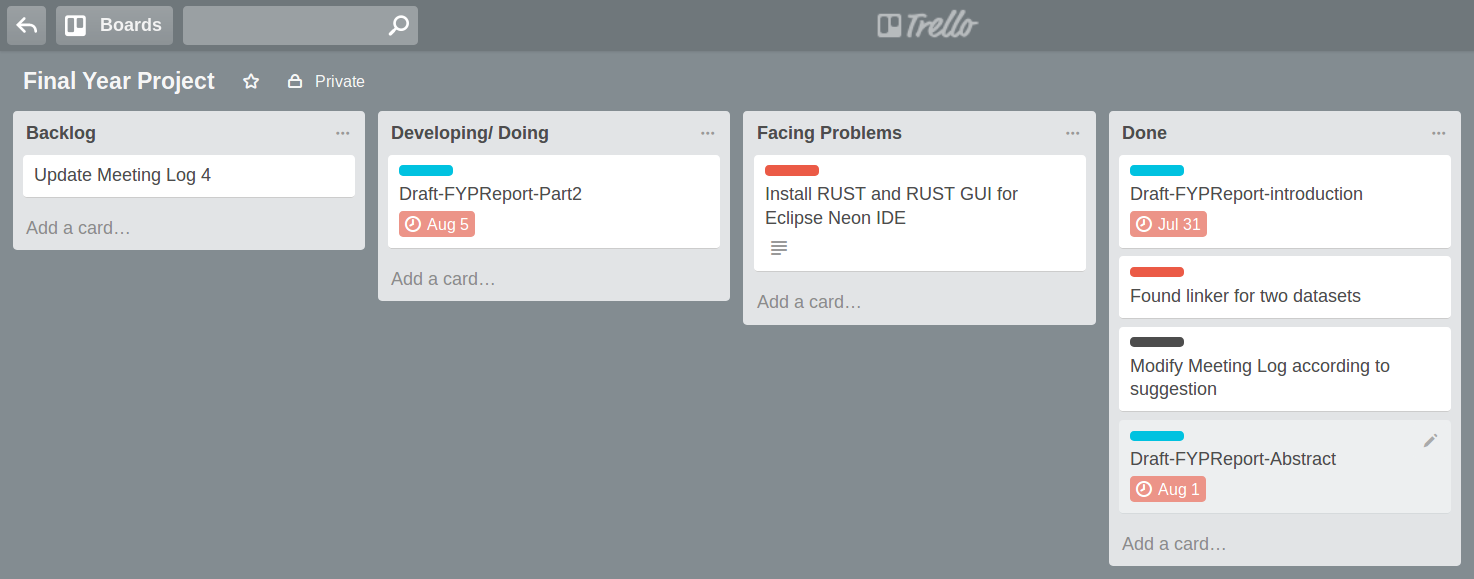
\includegraphics[width=1.0\textwidth]{Figure/kanban.png}
	\rule{35em}{0.5pt}
	\caption[Kanban board]{Kanban board}
\end{figure}

Kanban provide visual information of workflow by using sticky notes on a whiteboard to create a “picture” of our work. The board allow visualize the project development process or work flows within process and it helps ease the communicate status but also give and receive context for the work. Trello is used in this project as online Kanban board to manage the task in this methodology. 

There are an amount of work-in-progress (WIP) on each simple phased process to prevents overproduction and reveals bottlenecks dynamically to aware several roles whether are in bottlenecks. As an example, if the software pipelines are Backlog, Developing, Facing Problems and Done. There are WIP limits on each phased to increase the inspection and create awareness in order to facilitate adaptation based on the work loads. 

When a new requirement or changes requested, the task is insert into the backlog. The priority of the task are influenced by time constraint and importance. Afterwards, the task will be move into “developing” to began construction of documentation or codes. Once the task is encountered difficulty and problem, it will move to “”facing problem”. Alternatively, the task will move to “done” once the task is completed and ready to submit or show to supervisor during meeting. 

The Kanban events required to developed immediately and unknown incident may interrupt the progress depends on project feedback and requirement needs. A new high priority fix or changes may requested and it will break off the current project flow. Kanban allow the project respond to change efficiently and provide continuous update on progress to supervisor in order to submit quality works at end of project phase.  


\subsection{Methodology for this Project}

In this project, we will be developing Go and Rust program for conduct concurrent and distributed programming. To achieve the required tasks, rapid communication and modification is conducted to improve quality of program and satisfy project objectives. Prototyping method and Kanban will be use in this project.  

\pagebreak

%MAIN SECTION ================================
\section{Project Infrastructure}

\subsection{List of Hardware Resources}

\begin{enumerate}[topsep=0pt,itemsep=-1ex,partopsep=1ex,parsep=1.5ex]
\item \textbf{64-bit Personal Computer.} This machine is used for research and development activities of this project. The details are tabulated and shown below: 

\end{enumerate}

\begin{figure}[H]
	\centering
	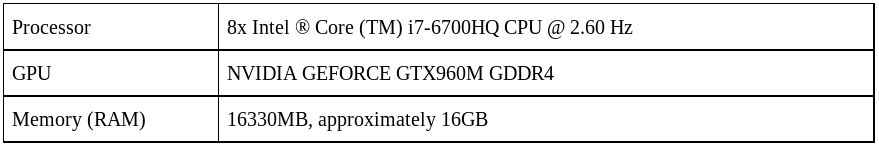
\includegraphics[width=1.0\textwidth]{Figure/computer-specs.png}
	\rule{35em}{0.5pt}
	\caption[Personal Computer Hardware table]{Personal Computer Hardware table}
\end{figure}

\subsection{List of Software Resources}

\begin{enumerate}[topsep=0pt,itemsep=-1ex,partopsep=1ex,parsep=1.5ex]

\item \textbf{Linux Ubuntu 16.04.3 LTS 64-bit.} The community driven and open source operating system is used to conduct concurrent and distributed computing with Go and Rust compiler installed. The details are discussed in Chapter 3.2.1. 

\item \textbf{Golang language compiler 1.8.3.} The linux amd64 gccgo compiler build Go source code into binary executable with “go build” and run the go program with “go run”. It is use to compile and run Go files this project.

\item \textbf{Rust language compiler 1.20.0. } The linux amd64 rustc compiler compile Go source code into executable with “rustc”.  It is use to compile Rust files in this project.

\item \textbf{PostgreSQL database 9.5.8.} The open source database management system is use for data handling and data storage for this project. The details are discussed in Chapter 3.2.3.

\item \textbf{Eclipse for Parallel Application Developers Oxygen Release (4.7.0) IDE.} The open source IDE provide perspective feature and integrated debugger to ease the coding and development activities for this project. The details are discussed in Chapter 3.2.2.

\item \textbf{Goclipse Plugin for Eclipse IDE.} The plugin provide debugging functionality, content assist, auto code indentation, open definition and integrated compiler for Go language on Eclipse IDE. 

\item \textbf{RUSTDT Plugin for Eclipse IDE.} The plugin provide syntax highlighting, error reporting, outline support, auto code indentation, debugging functionality and integrated compiler for Rust language on Eclipse IDE. 

\item \textbf{LTTng Tracing network. } The toolkits creating a tracepoint within Linux kernel, user application, libraries and output the traces into files. The details are discussed in Chapter 3.2.4.1.


\item \textbf{Eclipse Trace Compass.} The application view and analyze traces and produce useful graphical and tabulated information for debugging purposes. The details are discussed in Chapter 3.2.4.3.

\item \textbf{TeXstudio 2.10.8. } The software provide writing environment for create LaTeX document with numerous feature such as syntax-highlighting, reference checking with bibtex and various assistant. It is use for creating documentation for this project.
\pagebreak
\item \textbf{Visual Paradigm 14.1 free edition for non-commercial use.} The software is a free Unified Modelling Language Computer-Aided Software Engineering tool support 13 UML diagram types for software design and modelling. It is use to draw diagrams for this project. 

\end{enumerate}


\subsection{Other Project Resources}
\begin{enumerate}[topsep=0pt,itemsep=-1ex,partopsep=1ex,parsep=1.5ex]
	\item \textbf{Synaptic Package Manager. } The software system is a graphical package management program of APT libraries and provide same features as apt-get command. It provide great assist and help on managing software package dependencies. It is installed with \textit{“sudo apt-get install synaptic”} in terminal. 
	
	\item \textbf{Terminator.} Terminator provide multiple tabs, safe quit, UTF-8 encoding, automatic logging to ease the development activities for developer. The system is required to update source list with \textit{“sudo apt-get update”} and run \textit{“sudo apt-get install terminator”} to install the repository.
		
\end{enumerate}

\pagebreak

\subsection{Infrastructure Setup and Installation}

The required hardware and software resources are listed and discussed in Chapter 3.2, Chapter 4.2.1 and Chapter 4.2.2. 

\subsubsection{Go language compiler installation}

\begin{enumerate}[topsep=0pt,itemsep=-1ex,partopsep=1ex,parsep=1.5ex]
	\item Ensure Golang go1.8.3.linux-amd64.tar.gz is downloaded using wget in terminal. 
	\item Ensure downloaded file is extract, move and rename Golang directory. 
	\item Ensure Golang’s compiler export to system path. 
	\item Ensure Goroot and Gopath is set. 
	\item Ensure path to user profile .bashrc file is append. 
	\item Ensure Go executable and Go version installation is success. 
	\item Ensure Go libraries such as gocode, golint, guru, goimports, gorename and godef into Gopath directory are installed. 
	\item Ensure Godef Gometalinter is downloaded and executed. 
	
\end{enumerate}

The full installation steps for Go language compiler is found in Appendix A.1.
\pagebreak

\subsubsection{RUST language compiler installation}

\begin{enumerate}[topsep=0pt,itemsep=-1ex,partopsep=1ex,parsep=1.5ex]
    \item Install Rust toolchain with command line. 
    \item Export rust executable to system path. 
    \item Install Racer, Rustfmt, Rainicorn.
    \item Ensure all the required Rust executables are installed. 
	
\end{enumerate}

The full installation steps for RUST language compiler is found in Appendix A.2.

\subsubsection{Eclipse IDE installation}

\begin{enumerate}[topsep=0pt,itemsep=-1ex,partopsep=1ex,parsep=1.5ex]
    \item Ensure Java is installed before start download Eclipse.
    \item Run \textit{“sudo apt-get update”} and \textit{“sudo apt-get upgrade”} before start download. 
    \item Make eclipse-workspace folder as default storage for better management. 

\end{enumerate}

The installation details for Eclipse IDE is found in Appendix A.3.

\subsubsection{GoClipse plugin for Eclipse IDE installation}

\begin{enumerate}[topsep=0pt,itemsep=-1ex,partopsep=1ex,parsep=1.5ex]
	\item Install Goclipse plugin with Eclipse marketplace.
	\item Ensure Goclipse preferences and setting are correct.  
\end{enumerate}

The full installation steps for Goclipse plugin on Eclipse IDE is found in Appendix A.4.

\subsubsection{RustDT plugin for Eclipse IDE installation}

\begin{enumerate}[topsep=0pt,itemsep=-1ex,partopsep=1ex,parsep=1.5ex]
	\item Install RustDT plugin with Eclipse marketplace.
	\item Ensure RustDT preferences and setting are correct. 
\end{enumerate}

The full installation steps for RustDT plugin on Eclipse IDE is found in Appendix A.5.

\subsubsection{PostgreSQL database installation and setup}

\begin{enumerate}[topsep=0pt,itemsep=-1ex,partopsep=1ex,parsep=1.5ex]
	\item Install postgreSQL in command line. 
	\item Ensure database for FYP1 is created. 
	\item Create new user for database.
	\item Ensure database connection is established with user access.
\end{enumerate}

The full installation steps for PostgreSQL database is found in Appendix A.6.


% MAIN SECTION ===============================
%\section{Chapter Summary}
%Your job here
